\chapter{Background}
\label{ch:theoreticalbackground}
This research uses three main concepts of interest: the \textit{\gls{ps}}, \textit{\gls{antifragile}}, and \textit{\acrlong{ea}}. Understanding the interpretation of these concepts is essential for a \gls{sharedmentalmodel}. Besides the three main concepts, it is vital to understand the concept system. The three main concepts use \textit{system} as a concept. The concepts \textit{\gls{ps}}, \textit{\gls{antifragile}}, \textit{\acrshort{ea}}, and \textit{system} are defined for this \gls{sharedmentalmodel}.
\section{System}
\label{sec:tbsystem}
Literature often uses the same concept of system but with a different meaning \parencite[p.~37]{Lapalme2012}. System is used for many different things like software applications, interrelated people, systems of numerous interrelated elements (economical, socal, technological) and others \parencite[p.~37]{Lapalme2012}.

System has various definitions and types. E.g. open and closed, linear and nonlinear, dynamic and deterministic systems \parencite{Rickles2007}. A system can be an area of interest \parencite[p.~13]{Mannaert2016}. However, with another definition, a system is an object that is studied in the field \parencite[p.~933]{Rickles2007}. Both definitions are similar. The former acknowledged that the system is not isolated. The system of concern and systems in the environment have interactions \parencite[p.~13--14]{Mannaert2016}. This behaviour is what \textcite[p.~32]{Bertalanffy1968} calls an open system. An open system is a system that exchanges matter with its environment \parencite[p.~32]{Bertalanffy1968}, as where a closed system is considered to be isolated from its environment \parencite[p.~39]{Bertalanffy1968}.

A system is more than the sum of its parts. It is an indivisible whole \parencites[p.~51--69]{Ackoff1964}[p.~664]{Ackoff1973}. A system loses its essential properties when taken apart. The elements of a system can also themselves be systems. Every system can be a part of another system. These systems are also called sub-systems. This managerial idea of systems thinking is to focus on the interactions of the parts rather than their behaviour separately \parencite{Ackoff1964}. 

A mental model to understand a system is dependent on specific characteristics of the behaviour of a system. Understanding the behaviour of a system can only be in its environment \parencite[p.~29]{Gharajedaghi2011}. The boundary of a system is defined by the variables that can be influenced or controlled by the actors of that system \parencite[p.~182]{Gharajedaghi2011}. Variables that can not be influenced or controlled but impact the viability of the system are part of the context \parencite[p.~183]{Gharajedaghi2011} or the environment \parencite[p.~13--14]{Mannaert2016}. Understanding the environment will help to influence the environment. The \textit{Why they do} and \textit{What they do} of the actors in the environment help with influencing the environment \parencite[p.~33]{Gharajedaghi2011}. To understand the inner workings, one needs the ability to see complementary relations in opposing tendencies and to create feasible wholes with infeasible parts \parencite[p.~38]{Gharajedaghi2011}. However, the properties of a system are not the properties of its parts but that of the whole \parencites{Ackoff1973}{Gharajedaghi2011}. Because of these properties, actions intended to produce the desired outcome may generate opposite results, resulting in counter-intuitive behaviour \parencite[p.~48]{Gharajedaghi2011}.

The concepts of the \gls{ps}, \acrshort{ea} and \gls{antifragility} use different \glspl{specialisation} of the concept system. These \glspl{specialisation} are \textit{\acrfull{sos}}, \textit{\acrfull{sie}}, and \textit{Ecosystem}.
\subsection{System-of-Systems and System-in-Environment}
\label{sub:tbsysofsys}
A collection of independent systems that are part of a more extensive system has unique capabilities \parencite{INCOSE2018}. The independent systems working together have unique behaviour that they do not have on their own \parencite{INCOSE2018}.  A System-of-Systems is composed of multiple systems \parencites{Ackoff1973}{Gharajedaghi2011}. Using System-in-Environment stresses that a system is part of and should be aware of its environment \parencites{Gharajedaghi2011}{Lapalme2012}{Korhonen2016}{Mannaert2016}. Another variation is that of a System-in-Environment. System-in-Environment is a means to enforce environmental learning. With environmental learning, an enterprise adapts its desired goals to be more compatible with its environment \parencite[p.~41]{Lapalme2012}.
\subsection{Ecosystem}
\label{sub:tbecosystem}
The concept of ecosystem originated from the field of ecology. It was firstly defined by \textcite[p.~229]{Tansley1935} \parencite[p.~19]{Rich1988}. ''But the more fundamental conception is, as it seems to me, the whole system (in the sense of physics), including not only the organism-complex but also the whole complex of physical factors in the widest sense'', is the ecosystem as defined by \textcite[p.~299]{Tansley1935}. There are multiple transfers of the ecological ecosystem concept onto additional domains \parencite[p.~3]{Guggenberger2020}. A company must be viewed not as a member of a single industry but as part of a business ecosystem that crosses a variety of industries \parencite[p.~76]{Moore1993}. A business ecosystem is a concept that various businesses form value creation networks together \parencite[p.~3]{Guggenberger2020}. Ecosystems can be described as ''a set of actors with varying degrees of multilateral, non-generic complementarities that are not fully hierarchically controlled'' \parencite[p.~2255]{Jacobides2018}. There are different ways to order kinds of ecosystems. One way is that of dividing ecosystems into five specialisations. Business ecosystem \parencite[p.~76]{Moore1993}, platform ecosystem \parencite[p.~5]{Guggenberger2020}, service ecosystem \parencites{Barros2006}{Papazoglou2006}{Huang2014}, innovation ecosystem \parencites{Iansiti2004}{Carayannis2009}{Gomes2018}, and software ecosystem \parencites{Manikas2013}[p.~5]{Guggenberger2020} are possible specialisations \parencite[p.~5]{Guggenberger2020}.

The definitions of \acrlong{sos} and \acrlong{sie} are within the general definition of a system previously defined by \textcites{Ackoff1973}[p.~183]{Gharajedaghi2011}[pp.~13--14]{Mannaert2016}.
\section{Antifragile}
\label{sec:tbantifragile}
What is \gls{antifragile}, where did it originate, what can you achieve with it, and why is \gls{antifragile} important? These questions are the first things that come to mind when hearing \gls{antifragile} for the first time.

\Gls{antifragile} originated from the domain of risk management. \Gls{antifragile} was coined for the first time by \textcite{Taleb2012} as his answer to \glspl{blackswan} \parencite{Taleb2008}. \Glspl{blackswan} are large-scale unpredictable, and rare events of massive consequences \parencite[p.~6]{Taleb2012}. The rarer the event, the less tractable, and the less we know about how frequent its occurrence \parencite[p.~7]{Taleb2012}. The odds of rare events are not computable \parencite[p.~7]{Taleb2012}. ''Given the unattainability of perfect robustness, we need a mechanism by which the system regenerates itself continuously by using, rather than suffering from, random events, unpredictable shocks, \glspl{stressor}, and \gls{volatility}'' \parencite[p.~8]{Taleb2012}. With random events \gls{robust} is not good enough. Everything with the most minute vulnerability breaks. \Gls{robustness} cannot just be it, perfect \gls{robustness} is needed not to end up crashing the system \parencite[p.~8]{Taleb2012}. \Gls{fragile} systems fail when exposed to \glspl{stressor} \parencite[p.~21]{Ghasemi2017}. However, \gls{antifragile} systems prosper and improve in response to unpredictability, \gls{volatile}, randomness, chaos and disturbance \parencite[p.~21]{Ghasemi2017}. \Gls{antifragility} goes beyond \gls{resiliency} or \gls{robustness} \parencite[p.~21]{Ghasemi2017} (\cref{fig:eaal-triad}).
\begin{figure}[H]
	\centering
	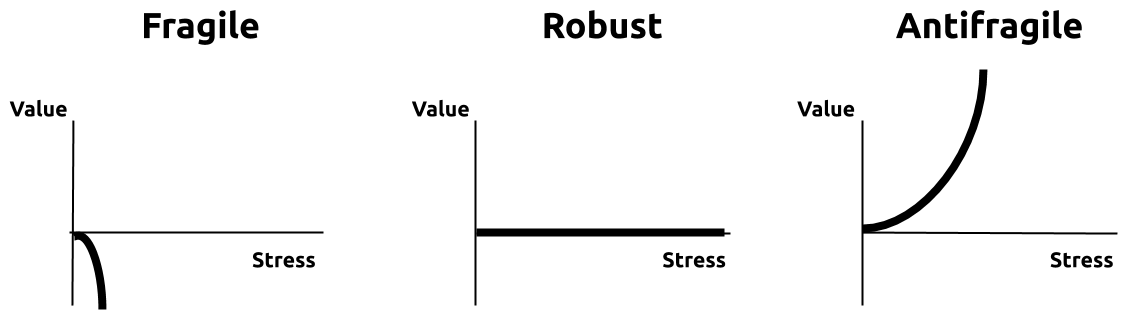
\includegraphics[width=0.8\linewidth]{images/eaal-triad}
	\caption[Triad of fragile, robust, and antifragile \parencite{Botjes2021}]{Triad of fragile, robust, and antifragile \parencite{Botjes2021}}
	\label{fig:eaal-triad}
\end{figure}
\Gls{antifragile} means that a system gains more than it loses. Positive asymmetry is achievable by reducing possible losses \parencite[p.~942]{Russo2017}. Reducing possible losses will reduce the harmful effects of exposure to damaging elements such as \glspl{stressor} and \gls{blackswan} \parencite[p.~942]{Russo2017}. \Gls{fragility} and \gls{antifragility} mean potential gain or harm from exposure to something related to \gls{volatility} \parencite[p.~13]{Taleb2012}. That something is what \textcite{Taleb2012} calls a member of the extended disorder family. This disorder family consists of \gls{uncertainty}, variability, imperfect, incomplete knowledge, chance, chaos, \gls{volatility}, disorder, \gls{entropy}, time, the unknown, randomness, turmoil, \glspl{stressor}, error, dispersion of outcomes, unknowledged \parencite[p.~13]{Taleb2012}. The disorder family is interpreted by \textcite[p.~12]{Botjes2020}, based on the works of \textcites[p.~436]{Taleb2012}[p.~3]{Gorgeon2015}, as \acrlong{vuca} from \textcite{Bennis1985}. \Gls{antifragility} is not only an answer to a \gls{blackswan} but also to random events, unpredictable shocks, \glspl{stressor}, and \gls{volatility} \parencite[p.~8]{Taleb2012}.
\subsection{Stressor}
\label{sub:backgroundstressor}
Publications on the subject of \gls{antifragile} often use \textit{\gls{stressor}} \parencite[p.~32]{Botjes2020}. What is a \textit{\gls{stressor}}? \textcite[p.~23]{Ghasemi2017} defined \textit{\gls{stressor}} based on \textcites{TurnerII2003}{Chrousos2009} as ''When systems are performing effectively, they are in a predetermined condition and conversely when they are not functioning correctly, they are in an unintended state. An unintended condition can be known or unknown. \textit{\Glspl{stressor}} are forces that threaten to transfer a system from an intended to an unintended condition.''
\subsection{Antifragile as a system property}
\label{sub:backgroundafpropertyofsystem}
A diversity of researchers define that \gls{fragility}, \gls{robustness} and \gls{antifragility} are properties of a system, like \textcites{Jaaron2014}{Kastner2017}{OReilly2019}{Botjes2021}. It is important to realise that the degree of \gls{antifragility} of a system is often a function of its internal structure \parencite[p.~886]{OReilly2019}. The ability to change under stress is governed by the interconnectedness of its sub-systems, how \gls{looselycoupled} those sub-systems are and how much of a change ripples trough the system \parencite[p.~886]{OReilly2019}. \Gls{selforganisation}, ownership, \gls{diversity}, \glspl{sharedmentalmodel} and a shared vision are some of the properties that an \gls{antifragile} system should posses \parencites{Jaaron2014}{Hole2016}{Kastner2017}{OReilly2019}{Botjes2021}. \textcite{Botjes2021} conducted extensive research to define \gls{antifragility} and the application of \gls{antifragility} on organisation design. \textcite{Botjes2021} used multiple sources (\cref{tab:tbsourcesofantifragileattributes}) to define a list of attributes.
\begin{longtable}{p{.4\textwidth}p{.4\textwidth}}
	\toprule%
	\multicolumn{2}{c}{\textbf{Sources used by \textcite{Botjes2021}}} \\%
	\midrule%
	\endhead%
	\hline
	\endfoot%
	\caption[Sources used for antifragile attributes]{Sources used for antifragile attributes}
	\label{tab:tbsourcesofantifragileattributes}
	\endlastfoot%
	\textcite{Ghasemi2017} & \textcite{Johnson2013} \\%
	\textcite{Kennon2015} & \textcite{Markey2018} \\%
	\textcite{Hendriksson2016} & \textcite{Kastner2017} \\%
	\textcite{Gorgeon2015} & \textcite{Hole2016} \\%
	\textcite{OReilly2019} & \\%
	\bottomrule%
\end{longtable}
The result of \textcite{Botjes2021} is the \acrfull{eaal} (\cref{fig:eaalbw}). The \acrfull{eaal} of \textcite{Botjes2021} is recent. \textcite{Botjes2021} used a data set collected by \textcite{Botjes2020}. \textcite{Botjes2020} created the data set through extensive literature research, but it only covers literature until June 2019 \parencite[p.~5]{Botjes2021}. 
\begin{figure}[H]
	\centering
	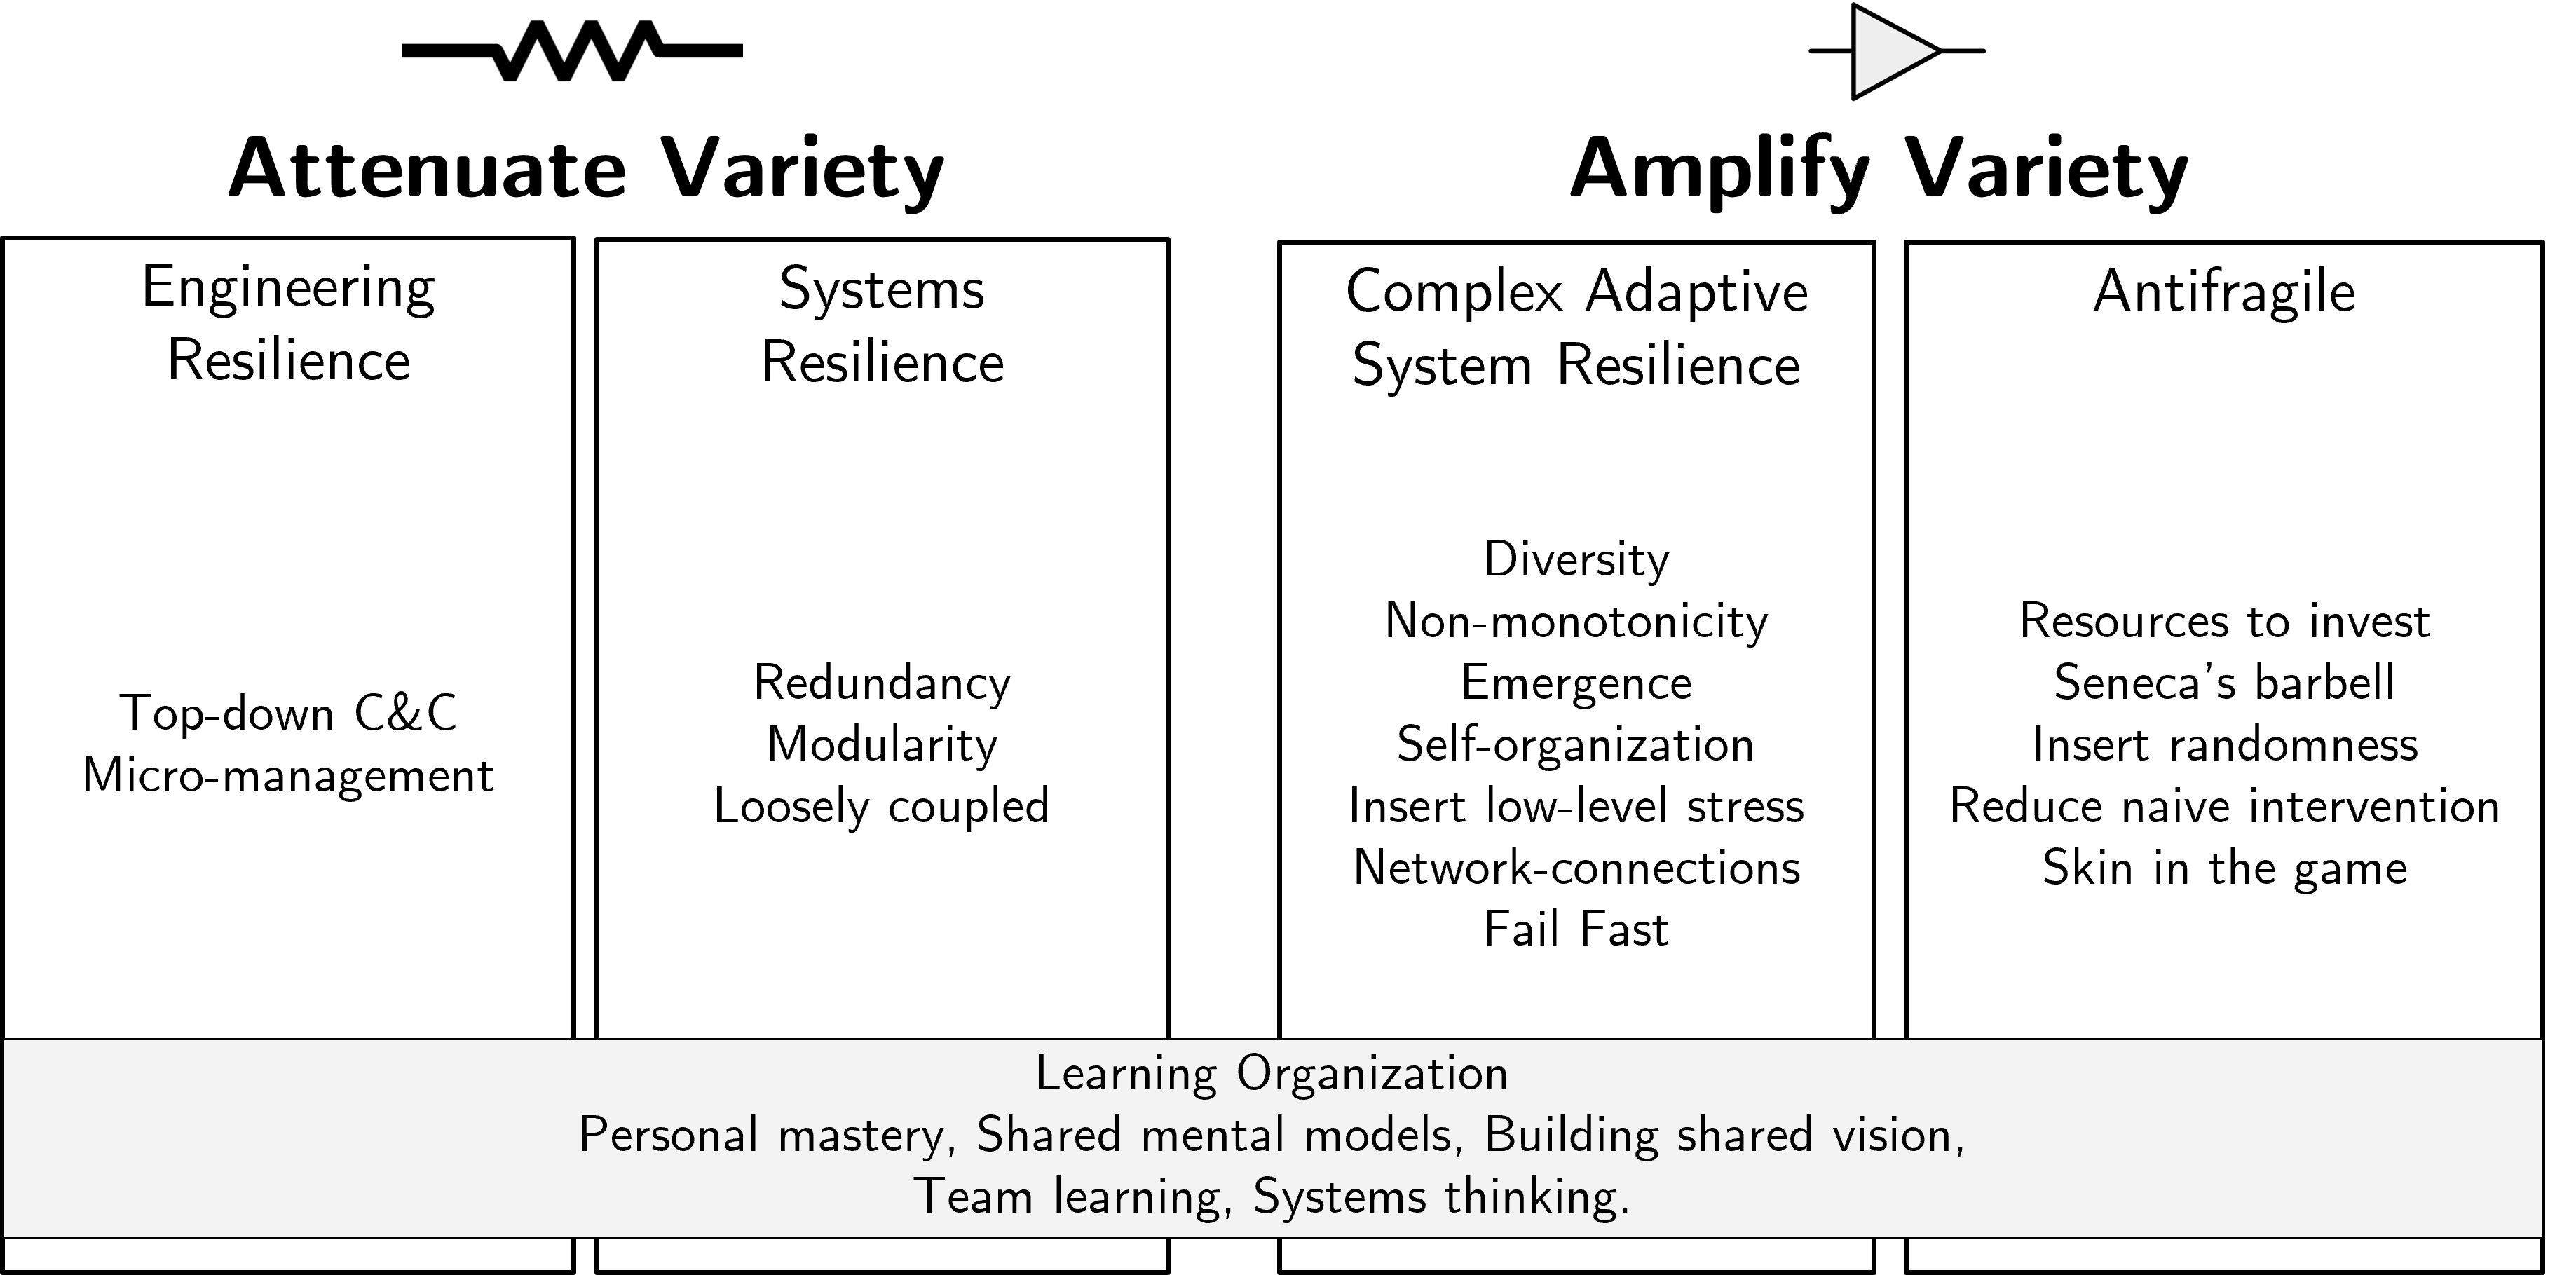
\includegraphics[width=0.8\linewidth]{images/eaalbw}
	\caption[Extended Antifragile Attribute List \parencite{Botjes2021}]{Extended Antifragile Attribute List \Parencite{Botjes2021}}
	\label{fig:eaalbw}
\end{figure}
Searching for \textit{new} literature makes sure that \textcite{Botjes2021} is recent and is not rebutted. Using the time frame of June 2019 until April 2022 makes sure that only new literature is found. The result of the search was thirty-one new sources. These sources are new articles, books and in-proceedings (\cref{app:literaturecatchup}). Of those thirty-one new sources, three were already in the literature set of \textcite{Botjes2020}. Eight were not found or publicly available, and thirteen were not relevant. Only seven were of interest to look at. After finalising the research, none of the literature added something new or rebutted the work of \textcite{Botjes2020}. \textcite{Botjes2021} is recent and contains \glspl{attribute} for a system, \acrlong{sos}, and a \acrlong{sie} to become more \gls{antifragile}.

The \acrlong{eaal} classifies \glspl{attribute} in two primary and five secondary categories. \textit{\Gls{attenuatevariety}} and \textit{\gls{amplifyvariety}} are the two primary categories. The five secondary categories are \textit{\gls{engineeringresilience}}, \textit{\gls{systemsresilience}}, \textit{\gls{casresilience}}, \textit{\gls{antifragile}} and \textit{learning organisation}. The \acrlong{eaal} does not contain resilience as a secondary category but multiple types of resilience. The \acrlong{eaal} assigned the secondary categories to the primary categories. \textit{\Gls{engineeringresilience}} and \textit{\gls{systemsresilience}} are assigned to \textit{\gls{attenuatevariety}}, while \textit{\gls{casresilience}} and \textit{\gls{antifragile}} to \textit{\gls{amplifyvariety}}. \textit{Learning organisation} is the only category assigned to both \textit{\gls{attenuatevariety}} and \textit{\gls{amplifyvariety}}.
\subsection{Resilience}
\label{sub:tbresilience}
\Gls{resiliency} is mentioned often in relation to \gls{antifragility}. \textcite[p.~3]{Botjes2021} uses the definitions of \textcite[pp.~5--8]{MartinBreen2011}. \textcite[pp.~5--8]{MartinBreen2011} identified several types of resiliency. These types are  \textit{\gls{engineeringresilience}}, \textit{\gls{systemsresilience}}, and \textit{\gls{casresilience}}. The definitions of \gls{resiliency} (\cref{tab:resiliencetypes}) have focus on the avoidance of harmful \glspl{stressor} and failure, including \gls{uncertainty} and \gls{volatility} \parencite[pp.~5--8]{MartinBreen2011}.
\begin{longtable}{p{.3\textwidth}p{.55\textwidth}}
	\toprule%
	\textbf{Type} & \textbf{Description} \\%
	\midrule%
	\endhead%
	\hline
	\endfoot%
	\caption[Types of resilience \parencite{MartinBreen2011}]{Types of resilience \parencite{MartinBreen2011}}
	\label{tab:resiliencetypes}
	\endlastfoot%
	\Gls{engineeringresilience} & Bounce back faster after stress, enduring greater stresses, and being disturbed less by a given amount of stress. \\%
	\Gls{systemsresilience} & Maintaining system function in the event of a disturbance. Systems resilience has been applied in governance and management, where it is often called robustness. \\%
	\Gls{casresilience} & The ability to withstand, recover from, and reorganise in repsonse to crisis. The function is maintained by the system structure may not be. The main differentiator is the adaptive capacity or adaptability of the system.\\%
	\bottomrule%
\end{longtable}
\subsection{Learning organisation}
\label{sub:learningorganisation}
\begin{wrapfigure}{r}{0.3\textwidth}
		\centering
		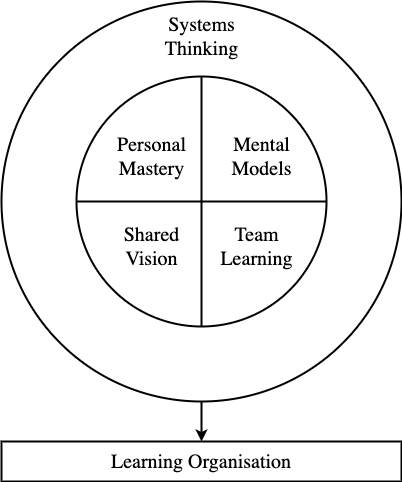
\includegraphics[width=\linewidth]{images/fithdiscipline}
		\caption[The fifth discipline]{The fifth discipline}
		\label{fig:fithdiscipline}
\end{wrapfigure}
One of the secondary categories of \acrlong{eaal} is learning organisation. But what is the learning organisation? The learning organisation is a way to create resilient organisations. These resilient organisations can cope better with unknown and unpredictable evens. ''Continuous improvement requires commitment to learning.'' \parencite{Garvin1993}. The learning organisation is an organisation that is equipped for creating, acquiring, and transferring knowledge \parencite{Garvin1993}. The result of this is that a learning organisation can modify its behaviour to reflect new knowledge and insights \parencite{Garvin1993}. \textcite{Senge1994} defined the \glspl{attribute} of the learning organisation that \textcite{Botjes2021} used in \acrlong{eaal} (\cref{fig:fithdiscipline}). These attributes are \textit{\gls{personalmastery}}, \textit{\glspl{sharedmentalmodel}}, \textit{\gls{buildingsharedvision}}, \textit{\gls{teamlearning}}, and \textit{\gls{systemsthinking}}.
\subsection{Attenuate variety and amplified variety}
\label{sub:attenuatevsaplify}
The two main categories in the \acrlong{eaal} are \gls{attenuatevariety} and \gls{amplifyvariety}. What is \gls{attenuatevariety} and \gls{amplifyvariety}? Variety originated from Cybernetics and was coined by \textcite{Ashby1956}. Variety denotes the count of states of a system \parencites{Ashby1956}{Ashby1958}. "Ashby and Beer stated the Law of Requisite Variety as 'variety can destroy variety ' \parencite[p.~207]{Ashby1956} and 'variety absorbs variety' \parencite[p.~286]{Beer1979}.'' \parencite[p.~31]{Botjes2020}. \textcite{Heylighen2001} described it with one single statement: ''If a system is to be stable, the number of states of its control mechanism must be greater than or equal to the number of states in the system being controlled.'' But what about the types of attenuate and amplify? \Gls{attenuatevariety} is reducing the variety in a system, while \gls{amplifyvariety} is increasing the variety in a system. ''To amplify internal variety is about increasing the chance of a higher \gls{entropy} and, therefore, more capable of absorbing the increasing external variety caused by change.'' \parencite[p.~31]{Botjes2021}. \Gls{attenuatevariety} is about increasing the chance of a lower \gls{entropy} and, therefore, less capable of absorbing increasing external variety caused by change \parencite[p.~31]{Botjes2021}. \Gls{engineeringresilience} and \gls{systemsresilience} result from \gls{attenuatevariety}, while \gls{casresilience} and \gls{antifragile} are a result of \gls{amplifyvariety} \parencite[p.~31]{Botjes2021}. Another interpretation is possible. \Gls{attenuatevariety} increases the \gls{fragility} of a system, while \gls{amplifyvariety} decreases the \gls{fragility} and increases the \gls{antifragility} of a system.
\subsection{Is agility antifragility?}
\label{tb:antifragile_vs_agility}
What is the relation between \gls{agile} and \gls{antifragile}? Is \gls{agile} \gls{fragile}, \gls{robust} or \gls{antifragile}? This question is improperly framed according to \textcite[p.~6]{Tomov2019}. \Gls{agility} can be \gls{fragile}, \gls{robust} or \gls{antifragile}. \Gls{antifragility} and \gls{robustness} are mathematically defined as properties, while \gls{agility} is not \parencite[p.~6]{Tomov2019}. \textcite[Abstract]{OReilly2019} states that rather than aiming to control or to remove control, we have to build systems, both technical and business, that aim to be \gls{antifragile} to change. By architecting \gls{antifragility}, businesses can gain \gls{agility}. We must build systems that aim to be \gls{antifragile} to change is better than trying to control change \textcite[abstract]{OReilly2019}. It results in the possibility of creating business and technical architectures that enable \gls{agility} through design. \textcite[p.~7]{Aghina2018} defined five trademarks and twenty-three practices for organisational \gls{agility}. When you combine these trademarks and practices with the \acrlong{eaal} of \textcite[p.~69]{Botjes2020} it is clear that the result is the same as that of \textcite[Abstract]{OReilly2019} who states \textit{\Gls{agility} through \Gls{antifragility}}. By using the attributes from the \acrlong{eaal} it is possible to achieve \gls{agility} in a system,. \Gls{agility} can be the result of applying \gls{antifragile} \glspl{attribute}. \Gls{agility} is a result of implementation, while \gls{antifragile} is a properties of a system.
\subsection{Antifragile system attributes}
\label{sub:attributesofantifragile}
The \acrlong{eaal} is selected as a source and starting point for \gls{antifragile} attributes (\cref{sub:backgroundafpropertyofsystem}). \Gls{optionality} is stated as an essential attribute by \textcites{Taleb2012}[p.~64]{Botjes2020}. \Gls{optionality} is excluded from the \acrlong{eaal} because of the overlap with \gls{diversity} \parencite[p.~64]{Botjes2020}. But \textcites{Taleb2012}[p.~9]{Gorgeon2015} both use the term \gls{optionality}. \Gls{optionality} is an idea advanced by \textcite{Taleb2012}. At the most basic level, \gls{optionality} means having lots of options. The difference between \gls{optionality} and \gls{diversity} is very subtle. \Gls{optionality} allows the buyer to retain the upper bound and be unaffected by adverse outcomes which makes the buyer \gls{antifragile}\footnote{\label{foot:nesslabs}\url{https://nesslabs.com/optionality-fallacy}}. Despite the minimal difference between \gls{optionality} and \gls{diversity}, \gls{optionality} can still have a distinctive character in the \gls{ps}. Adding \gls{optionality} to the already defined set of the \acrlong{eaal} brings a total of twenty-three attributes. The \acrlong{eaal} categorised the attributes into \gls{attenuatevariety}, \gls{amplifyvariety}, and \gls{learningorganisation}. Adding \gls{optionality} to \gls{amplifyvariety} makes it equal to \gls{diversity}. For the overview of the \glspl{attribute} for \gls{antifragile} see \cref{tab:attributesofantifragile}. 
\begin{longtable}{@{}p{.4\textwidth}p{.4\textwidth}@{}}
	\toprule%
	\textbf{Attribute} & \textbf{Category} \\%
	\midrule%
	\endhead%
	\hline
	\endfoot%
	\caption[Antifragile system attributes]{Antifragile system attributes}
	\label{tab:attributesofantifragile}
	\endlastfoot%
	\Gls{topdowncc} & \Gls{attenuatevariety} \\%
	\Gls{micromanagement} & \Gls{attenuatevariety} \\%
	\Gls{redundancy} & \Gls{attenuatevariety} \\%
	\Gls{modularity} & \Gls{attenuatevariety} \\%
	\Gls{looselycoupled} & \Gls{attenuatevariety} \\%
	\Gls{diversity} & \Gls{amplifyvariety} \\%
	\Gls{nonmonotonicity} & \Gls{amplifyvariety} \\%
	\Gls{emergence} & \Gls{amplifyvariety} \\%
	\Gls{selforganisation} & \Gls{amplifyvariety} \\%
	\Gls{insertlowlevelstress} & \Gls{amplifyvariety} \\%
	\Gls{networkconnections}  & \Gls{amplifyvariety} \\%
	\Gls{failfast} & \Gls{amplifyvariety} \\%
	\Gls{resourcestoinvest} & \Gls{amplifyvariety} \\%
	\Gls{senecabarbell} & \Gls{amplifyvariety} \\%
	\Gls{insertrandomness} & \Gls{amplifyvariety} \\%
	\Gls{reducenaiveintervention} & \Gls{amplifyvariety} \\%
	\Gls{skininthegame} & \Gls{amplifyvariety} \\%
	\Gls{optionality} &  \Gls{amplifyvariety} \\%
	\Gls{personalmastery} &  \Gls{learningorganisation} \\%
	\Gls{sharedmentalmodel} &  \Gls{learningorganisation} \\%
	\Gls{buildingsharedvision} &  \Gls{learningorganisation} \\%
	\Gls{teamlearning} &  \Gls{learningorganisation} \\%
	\Gls{systemsthinking} &  \Gls{learningorganisation} \\%
	\bottomrule%
\end{longtable}

\section{Public sector}
\label{sec:tbpublicsector}
The context of this research is the public sector. We need to define the public sector to have a common understanding that will help to place this research in its proper context. However, we will not explain how the public sector functions in the Netherlands in detail.

The public sector is the collective name for all government and semi-government organisations. We divide the governments into three levels: the national government, the regional government, and the local government \parencite{PrivacySense2016}. We see these levels also in the Dutch public sector: the national government, the provinces, and the municipalities \parencite{Overheidsvormen}. The Netherlands is a decentralised unitary state \parencite[p.~10]{Libert2016}. A decentralised unitary state is a form of government in which territorial units within a unitary state have independent powers \parencite{Grondwetb}. The organisation of local and regional authorities is formalised in the Netherlands by the Provinces Act and the Municipalities Act \parencite{Grondwet}. Provinces and municipalities can therefore decide on issues themselves. There is no fixed demarcation of tasks between the levels of the government \parencite{Grondwet}. 

Nevertheless, provinces and municipalities have a general power to regulate and manage, which can only be limited by law. However, provinces and municipalities are obliged to cooperate in implementing rules set by higher authorities. They can by law be subject to supervision \parencite{Grondwetb}.

My observation is that, as a result, there are differences in implementing laws between municipalities themselves and between provinces. One municipality is helping people get financially healthier by coaching while another municipality s employing residents. It is about law for social benefits in both cases—two different implementations of the same law.

The national government is the part of the government that works at the national level. They are responsible for policy-making, passing laws and monitoring compliance. In addition, the central government is responsible for preparing plans for the government and parliament and carrying out these plans \parencite{Takenrijksoverheid}.  The provinces can decide independently on many matters. E.g. the creation of new nature and building new roads. In addition, the provinces also implement several national laws \parencite{Takenprovincie}. Municipalities only perform tasks that are of direct importance to their residents. Making those choices is the essential task of a municipal council. In addition, the municipalities also implement many national laws. For example, every municipality must issue passports and identity cards to its residents \parencite{Takengemeente}. 

The national government consists of 12 ministries \parencite{Rijksoverheid}, which include approximately 160 organisations. There are 12 provinces \parencite{Overheidsvormen} and 344 municipalities \parencite{Herindeling}. Organisations that are part of the public sector but are not classified as an organisation belonging to one of the three levels are excluded from this count. 

% When we define the public sector as a system you have a system of systems. The system can be the public sector with the central government, provinces and municipalities as sub-systems.

\subsection{Differences with the Private Sector Market}
\label{sub:tbdifferenceprivatesector}
What makes the \gls{ps} different from the private sector? What is the main distinction? This answer is in the core values of both sectors. \Textcite{Wal2008} states that the top five private sector core values are profitability, accountability, expertise, reliability, and effectiveness. While \textcite{Wal2008} states that the top five \gls{ps} core values are accountability, effectiveness, incorruptibility, reliability, and lawfulness. Profitability is only a value for the private sector, and it does not exist as a value for the public sector \parencite{Wal2008}. The \gls{ps} demands or even initiates changes without noticing the needed investments to execute these changes by the private sector.


% Public accountability is a huge difference! 

Public accountability is a form of accountability that relates specifically to the public sector. Public accountability as such should be distinguished from public responsibilities, which involves a substantive discussion about tasks, obligations and liabilities in the public sector.

Elements:

Accountability relates to the expenditure of public funds
Accountability relates to the exercise of public duties and powers
Accountability is public
Accountability is placed in the perspective of the public good




I will focus this research on the public sector level local government of the Netherlands. In \cref{sec:discussions} I will discuss the applicability on non Dutch public sectors.


\subsection{Collaboration between public and private sector}

More often the public sector is partnering with a privatly held organisation to create a public-private partnership or \acrfull{jv}. These hybrid organisations work together to deliver a service or business venture to a community jointly. Through outsourcing, public sector organisations will often engage the private sector to deliver goods and services to their citizens. 

\begin{figure}[H]
	\centering
	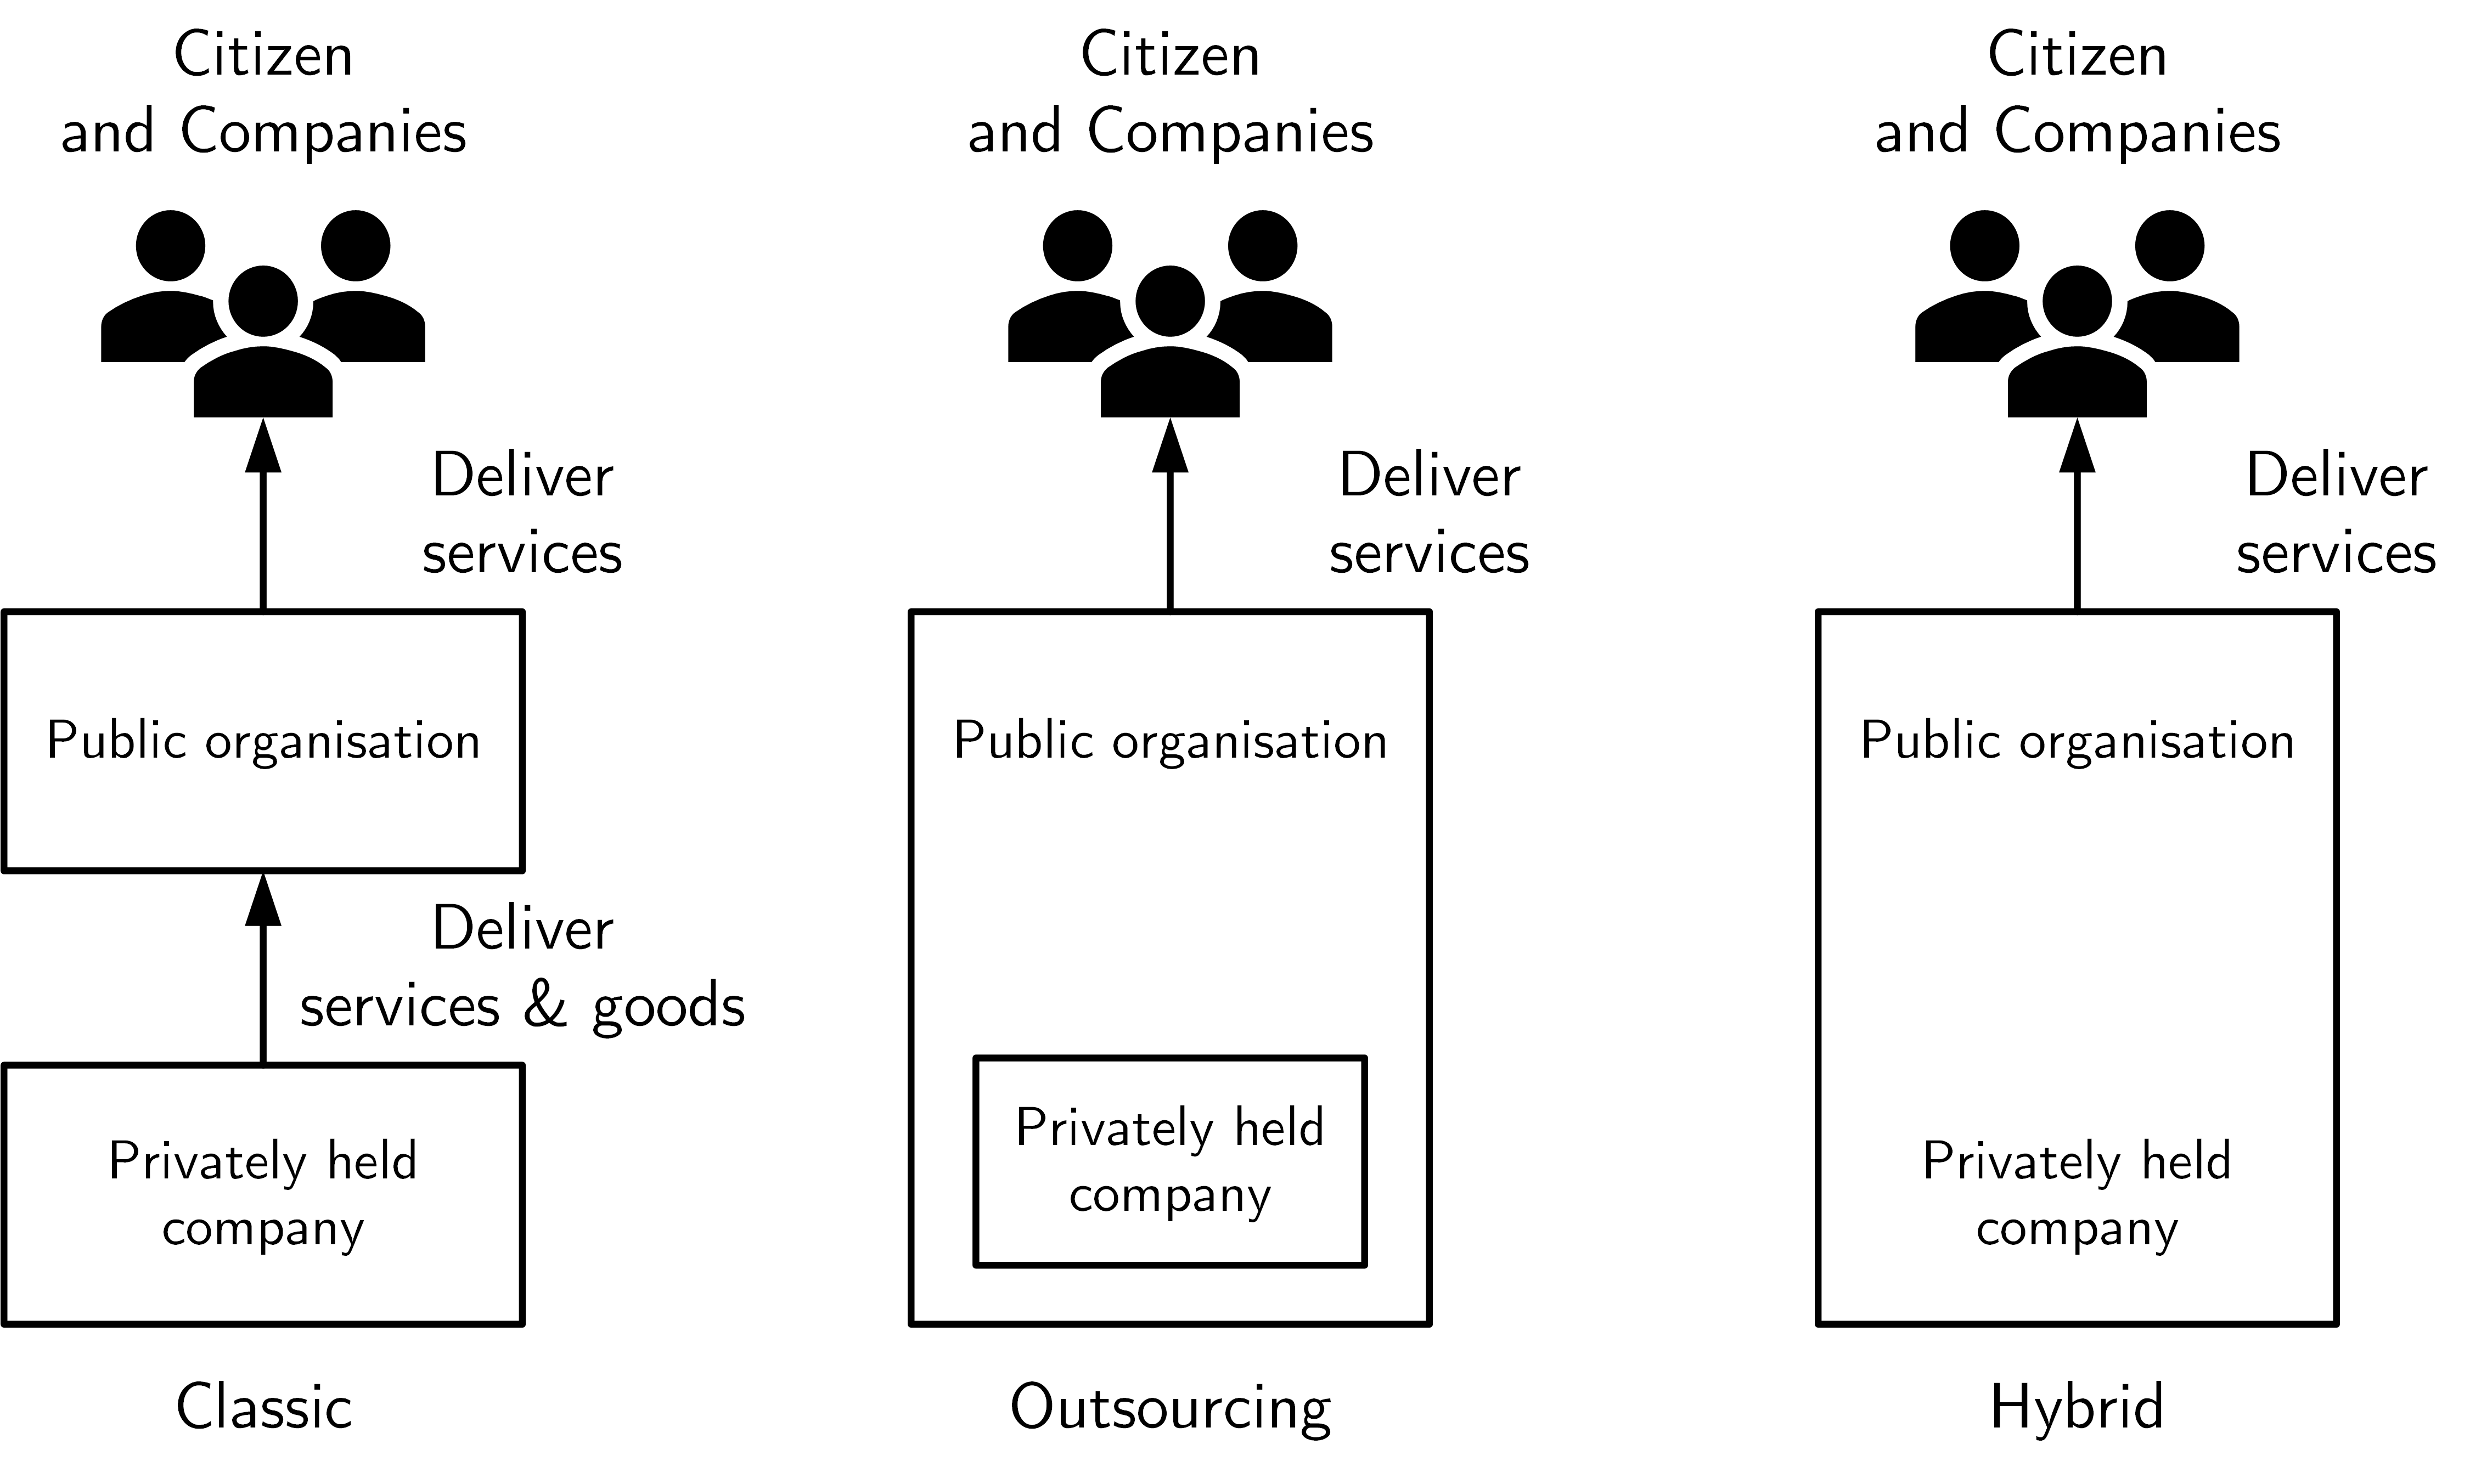
\includegraphics[width=0.7\linewidth]{images/publicsector3modelsofcolaboration}
	\caption[Public sector collaboration models]{Public sector collaboration models}
	\label{fig:publicsector3modelsofcolaboration}
\end{figure}

I argue that, in the hybrid model, the definition of the public sector is not correct anymore. The part of a private company that is a part of a hybrid collaboration, in a \gls{jv}, with the public sector should be part of the public sector system.

Themes relevant for the government for 2021 until 2025 (i-Strategy) \parencite{Digitaleoverheid}.

\begin{enumerate}
	\item{I in het hart}
	\item{Digitale weerbaarheid}
	\item{ICT-landschap}
	\item{Generieke voorzieningen}
	\item{Informatiehuishouding}
	\item{Data en Algoritmen}
	\item{I-vakmanschap}
	\item{Transparantie en inzicht}
	\item{I-besturing}
	\item{Markt en innovatie}
\end{enumerate}



\subsection{The public sector as a System of Systems}
\label{sub:tbpssystemofsystems}

\begin{figure}[H]
	\centering
	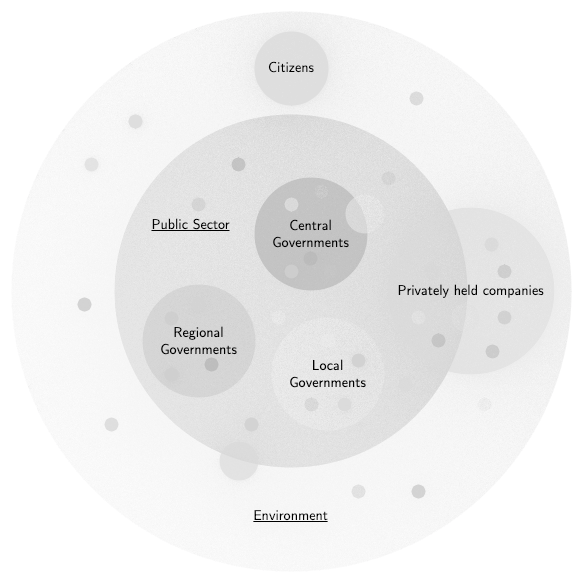
\includegraphics[width=0.5\linewidth]{images/pssystemofsystems}
	\caption[Public Sector as a \acrlong{sos}]{Public Sector as a \acrlong{sos}}
	\label{fig:pssystemofsystems}
\end{figure}

\section{Enterprise Architecture}
\label{sec:tbenterprisearchitecture}
This research is about which success factors positively influence \acrfull{ea} in achieving \gls{antifragility} in the \gls{ps}. This statement already assumes that \acrshort{ea} is a means to achieve a goal. Is this correct? Does the world have the same idea about \acrshort{ea}, or do they see it differently? Can \acrshort{ea} contribute to reaching the goals of an organisation or even a system? Regardless of the attention \acrshort{ea} gets, many researchers and practitioners have indicated that there is a lack of a shared mental model \parencite[p.~2]{SaintLouis2019}. The various definitions are not always complimentary, and sometimes they are even opposite \parencites{Hoogervorst2009}{Lapalme2012}{SaintLouis2019}. A lens on Enterprise Architecture needs to be defined for this research to create a shared understanding of Enterprise Architecture. There is no shared mental model of Enterprise Architecture \parencite[p.~2]{SaintLouis2019}. The lack of a shared mental model can create confusion and conflicts concerning the purpose of Enterprise Architecture and its practice \parencite[p.~1]{SaintLouis2019}. The definitions vary in the scope of application. Some definitions only focus on IT systems, while others focus on the business, the enterprise, the environment, or any other combination. E.g. the definitions from \textcites{Gartner}{Graves2009}{Ross2014}{White2018}.
\vskip\baselineskip
\noindent \underline{Definition of \textcite{Gartner}}: \acrlong{ea} analyses the execution of change toward a desired business vision and outcomes. \acrlong{ea} leads the enterprise proactively and holistically, responding to disruptive forces.
\vskip\baselineskip
\noindent \underline{Definition of \textcite[p.~5]{Graves2009}}: \acrlong{ea} is the organising logic for business processes and IT infrastructure, reflecting its operating model's integration and standardisation requirements. It provides a long term view of a company's processes, systems and technologies so that individuals can build capabilities and not just fulfil immediate needs.
\vskip\baselineskip
\noindent \underline{Definition of \textcite[p.~9]{Ross2014}}: \acrlong{ea} is the organising logic for business processes and IT infrastructure, reflecting its operating model's integration and standardisation requirements. It provides a long term view of a company's processes, systems and technologies so that individuals can build capabilities and not just fulfil immediate needs.
\vskip\baselineskip
\noindent \underline{Definition of \textcite{White2018}}: \acrlong{ea} is the process by which organizations standardize and organize IT infrastructure to aligns with business goals. These strategies support digital transformation, IT growth and the modernization of IT as a department. \acrshort{ea} is the practice of analysing, designing, planning and implementing enterprise analysis to successfully execute on business strategies. \acrshort{ea} helps to lay out how information, business and technology flow together.
\vskip\baselineskip
All four Enterprise Architecture definition examples provide decision-support for direction and change at any level of the enterprise. E.g. ''The choices in the journey of an enterprise for an executive, the preferred technologies of process models for new developments for programme and portfolio management, as well planning when to decommission, change or replace systems'' \parencite[p.~4]{Graves2009}. Mature \acrshort{ea} can map interdependencies across almost every aspect of the enterprise \parencite[p.~5]{Graves2009}. A well defined and maintained \acrshort{ea} is proven to be a critical factor in an organisation's agility, effectiveness and ability to respond to risk, opportunity and change \parencite{Ross2014}. Enterprise Architecture assists in managing changes imposed on the organisation from the outside, by the market, by regulations, or at an operations level, by system failures, environmental incidents or customer complaints \parencite[p.~5]{Graves2009}. \acrshort{ea} can support re-designs and re-organisation, especially during significant organisational changes, mergers or acquisitions \parencite{White2018}. System development, IT Management, decision-making, and IT risk management are examples of capabilities supported by \acrshort{ea} \parencites{Graves2009}{Ross2014}{White2018}. Because a shared mental model is absent, there is also no clear approach to practising Enterprise Architecture \parencite[p.~2]{SaintLouis2019}.
\subsection{Approaches of Enterprise Architecture}
\label{sub:eaapproaches}
There are several perspectives to the practice of \acrshort{ea} \parencites{Lapalme2012}{Kotusev2015}{Ylinen2018}{Ylinen2020}. One of the perspectives is an approach that distinguishes two groups of \acrshort{ea} experts. A modelling-focused group forms a comprehensive view of an organisation, and a development-focused group using \acrshort{ea} for organisational development \parencites[p.~6]{Ylinen2020}. 
\begin{longtable}{p{.4\textwidth}p{.6\textwidth}}
	\toprule%
	\textbf{Approach} & \textbf{Description} \\%
	\midrule%
	\endhead%
	\hline
	\endfoot%
	\caption[Three approaches to Enterprise Architecture]{Three approaches to Enterprise Architecture}
	\label{tab:tbthreeapproaches}
	\endlastfoot%
	Traditional & A four-step sequential process. Document the current (as-is, baseline) state, develop the desired future (to-be, future) state and the transition plan to migrate from the current to the target state, and implement the plan and repeat the process. \\%
	\acrshort{mit} & Advocates the development of a long-term enterprise-level architectural vision to be translated into concrete project-level decisions through IT governance mechanisms. These decisions involve business and IT managers on different organisational levels. \\%
	\acrshort{dya} & ''Just enough, just in time'' architecture. The development of \acrshort{ea} starts no earlier than there is a need for it. Business initiatives trigger the activities of 
	\acrshort{ea} to make sure that needed projects fit nicely into the existing \acrshort{ea} and in the strategic plans of the enterprise. \\%
	\bottomrule%
\end{longtable}
However, another perspective distinguished three approaches \parencite[p.~4071]{Kotusev2015}. The traditional \parencite{Spewak1993}, the \acrfull{mit} \parencite{Ross2014}, and the \acrfull{dya} \parencite{Wagter2005} approach \parencite[pp.~4071--4072]{Kotusev2015} (\cref{tab:tbthreeapproaches}). When you scrutinise the definitions of the three approaches, it becomes clear that the approaches are focused on organisations and not the environment. The \acrshort{ea} three schools of thought from \textcite{Lapalme2012} gives another perspective. Three possible schools of thought in the practice of \acrshort{ea} are, \gls{enterpriseitarchitecting}, \gls{enterpriseintegrating}, and \gls{enterpriseecologicaladaptation} \parencite[pp.~38--41]{Lapalme2012} (\cref{tab:tbschoolsofthought,app:easchoolsproperties}).
\begin{longtable}{p{.4\textwidth}p{.6\textwidth}}
	\toprule%
	\textbf{Approach} & \textbf{Description} \\%
	\midrule%
	\endhead%
	\hline
	\endfoot%
	\caption[Enterprise Architecture schools of thought]{Enterprise Architecture schools of thought}
	\label{tab:tbschoolsofthought}
	\endlastfoot%
	\gls{enterpriseitarchitecting} & \acrshort{ea} is the glue between business and IT. \acrshort{ea} is an enabler for executing the business strategy. This school is about aligning an enterprise's IT assets to execute business strategy effectively and various operations using the proper IT capabilities. The school \gls{enterpriseitarchitecting} focuses on the IT capabilities while not questioning the business capabilities. \\%
	\gls{enterpriseintegrating} & \gls{enterpriseintegrating} links strategy and execution. It is not only enabling enterprise strategy it also implements it. Designing all the organisational dimensions is fostered with systems thinking. \gls{enterpriseintegrating} is aware of its environment and tries to manage the environment. \\%
	\gls{enterpriseecologicaladaptation} & \acrshort{ea} fosters organisational learning by designing all facets of the enterprise. It changes the environment and systematically designs the enterprise, including its relationship to the environment. The enterprise's relationship to its environment is an indisputably connected facet. This school of thought enables innovation and System-in-Environment adaptation. It looks for bidirectional incoherence between the enterprise and its environment. Nevertheless, it is the means for organisational innovation and sustainability. It is about enterprise and environment co-evolution. \\%
	\bottomrule%
\end{longtable}
\subsection{Defining Enterprise Architecture}
\label{sub:definingea}
\Gls{antifragile} deals with \glspl{stressor} and \glspl{blackswan} originating from the (environment of the) system of interest. The \acrlong{eaal} of \textcite{Botjes2021} fosters \gls{organisationallearning} and \gls{systemsthinking} capabilities to deal with \glspl{stressor} and \glspl{blackswan} \parencite[pp.~2--4]{Botjes2021}. Exploring the \acrlong{ea} schools of thought \parencite{Lapalme2012} makes it clear that \textit{\gls{enterpriseecologicaladaptation}} is the best school in the context of \gls{antifragility}. \textit{\gls{enterpriseecologicaladaptation}} has a clear focus on the environment, fosters organisational and \gls{environmentallearning}, and embraces \gls{systemsthinking} \parencite[pp.~40--41]{Lapalme2012}. Although the school \textit{\gls{enterpriseintegrating}} already has the notion of the environment, it is not changing the environment like the school \textit{\gls{enterpriseecologicaladaptation}}. At the same time, \textit{\gls{enterpriseitarchitecting}} has its main focus on the IT organisation of the enterprise itself. If an organisation want to survive in the turbulence of today's markets, the organisation must learn to adapt and innovate \parencite[p.~42]{Lapalme2012}. The school \textit{\gls{enterpriseecologicaladaptation}} is about adapt and innovate.

It is still necessary to define the definition of \acrshort{ea}. The lens of \acrshort{ea} is partly defined. \textit{'The how'} is known. The \acrlong{ea} school of thought \gls{enterpriseecologicaladaptation} is selected. The properties of this school are known (\cref{sec:propeea}). We still miss the definition of \acrshort{ea}. \textit{'The what'} is still unknown. \textcite[p~42]{Lapalme2012} mapped \acrlong{ea} authors and literature to the three schools of thought (\cref{app:easchoolsresearchers}).
\begin{table}[H]
	\centering
	\resizebox{\textwidth}{!}{%
	\begin{tabular}{p{0.4\textwidth}p{0.6\textwidth}}
		\toprule
		\textbf{Author(s)} & \textbf{Description} \\%
		\midrule
		\citeauthor{Gharajedaghi2011} & \textcite{Gharajedaghi2011}  is about systems theories and does not have its focus on \acrshort{ea}. \\%
		\citeauthor{Hoogervorst2009} & \textcite{Hoogervorst2009} is about Enterprise Governance and Enterprise Engineering. It addresses \acrshort{ea} and provides definitions. \acrshort{ea} is more a design discipline.  \\%
		\citeauthor{Graves2008} & \textcite{Graves2008} is about \acrshort{ea}, the goal and use of \acrshort{ea}, and it contains definitions of \acrshort{ea}. \\%
		\citeauthor{Martin1995} & \textcite{Martin1995}  is about aligning enterprise engineering to people, techology, and strategy. \acrshort{ea} is more a design discipline. \\%
		\citeauthor{Smith2011} & \textcite{Smith2011} is about an \acrshort{ea} framework. It does not contain definitions on \acrshort{ea}. \\%
		\citeauthor{Lapalme2012b} & \textcite{Lapalme2012b}  is not publicly available and accessible. It is about socio-technical systems strengthen \acrshort{ea}. \\%
		\bottomrule
	\end{tabular}
	}%
	\caption[Authors of Enterprise Ecological Adaptation]{Authors of Enterprise Ecological Adaptation}
	\label{tab:eeaauthors}
\end{table}
A definition of \acrlong{ea} must be aligned with the \acrlong{ea} school of thought of \gls{enterpriseecologicaladaptation}. Using the list of authors and sources for the school of thought of \gls{enterpriseecologicaladaptation} (\cref{tab:eeaauthors}) shows that two sources contain definitions of \acrlong{ea}. The first source that contains definitions is \textcite{Hoogervorst2009}. \textcite[p.~8]{Hoogervorst2009} defines \acrshort{ea} as something that provides normative guidance for design in order for the enterprise to operate satisfied. \acrshort{ea} comprises four sets of architecture business, organisation, information, and technology, which are associated with the corresponding enterprise design domains. 

The second is that of \textcite{Graves2008}. ''\acrlong{ea} is the integration of everything the enterprise is and does.'' \parencite[p.~1]{Graves2008}. \acrlong{ea} is about the structure of the whole of the enterprise—the whole rather than a single sub-system. There are no simple states of 'as is' and 'to be'. The world is dynamic and not static. Everything in a business system depends on everything else \parencite[p.~14]{Graves2008}.

\citeauthor{Graves2008}'s definition directly relates to the \acrlong{ea} school of thought of \gls{enterpriseecologicaladaptation} and \gls{antifragility}. This research uses the definition of \textcite{Graves2008} as a lens.
\subsection{Enterprise Architecture system attributes}
\label{sub:attributesonea}
The \acrlong{ea} school of thought of Enterprise Ecological Adaptation has the best alignment with \gls{antifragile} (\cref{sec:tbenterprisearchitecture}). The \glspl{attribute} used for \acrlong{ea} will be those of the school of \gls{enterpriseecologicaladaptation}.  It contains \glspl{attribute} related to learning and \gls{systemsthinking}. \Gls{organisationallearning}, \gls{environmentallearning}, and \gls{systeminenvironmentcoevolutionlearning} are related to learning and \gls{systeminenvironment}, \gls{holisticsystemicstance}, and \gls{intraorganisationalcoherency} to \gls{systemsthinking}. See for a full overview \cref{tab:attributesofeea}.
\begin{longtable}{@{}p{.4\textwidth}p{.4\textwidth}@{}}
	\toprule%
	\textbf{Attribute} & \textbf{Category} \\%
	\midrule%
	\endhead%
	\hline
	\endfoot%
	\caption[Enterprise Architecture system attributes]{Enterprise Architecture system attributes}
	\label{tab:attributesofeea}
	\endlastfoot%
	\Gls{systeminenvironment} & \Gls{enterpriseecologicaladaptation} \\%
	\Gls{holisticsystemicstance} & \Gls{enterpriseecologicaladaptation} \\%
	\Gls{intraorganisationalcoherency} & \Gls{enterpriseecologicaladaptation} \\%
	\Gls{organisationallearning} & \Gls{enterpriseecologicaladaptation} \\%
	\Gls{environmentallearning} & \Gls{enterpriseecologicaladaptation} \\%
	\Gls{systeminenvironmentcoevolutionlearning} & \Gls{enterpriseecologicaladaptation} \\%
	\bottomrule%
\end{longtable}